% !TeX root = ./thesis.tex










%==============================
\chapter{The Animat}
\label{ch:animat}


%-----
\section{The Digital Universe}
The first attempts to model artificial life date all the way back to the 1940s. It was then when John von Neumann, while researching advanced computer structures, based on parallel processing, laid the foundations of a special structure denoted as a \emph{cellular automaton}. Indeed, most of the early artificial life research was based on the cellular automaton, Conway's `Game of Life' \cite{gardner:1970} and Langton's self-reproducing loop \cite{langton:1984} being the most renown examples \cite{adami:1998,emmenche:1994,rucker:1993}.

The cellular automaton is formally defined as a \emph{spatial array} of \emph{cells}, where each cell holds a \emph{digital state number} \cite{rucker:1993}. The cells' states are updated in \emph{parallel} at \emph{discrete time steps}. In addition, it is required that the method of updating is \emph{local} and \emph{homogeneous}. In most cases the cells' next states are computed based on their current state and the state of their immediate neighbourhood (\ie\ the states of the cells that are, with respect to their spatial arrangement, adjacent to the observed cell). But the fixed topology of the cellular automaton makes it difficult to apply to modelling the dynamics of organized groups of moving animals. However, according to Mraz \cite{mraz:2000}, the abstract structure that is the most suitable for modelling a cell in the cellular automaton is the Moore automaton \cite{kohavi:1978}. 

\begin{definition}
\label{def:Moore}
	The Moore automaton is defined as a five-tuple $\langle\set{X},\set{Q},\set{Y},\delta,\lambda\rangle$, where $\set{X}$, $\set{Q}$ and $\set{Y}$ are non-empty sets representing the input alphabet, the internal states and the output alphabet respectively; $\delta$ is a mapping called the transition function and $\lambda$ is a mapping called the output function:
	\begin{eqnarray}
		& \delta: \set{X}\times \set{Q}\rightarrow \set{Q}, & \\
		& \lambda: \set{Q}\rightarrow \set{Y}. &
	\end{eqnarray}
	At any discrete time step $t \in \set{T}$, where $\set{T}$ is a non-empty set of discrete time steps, the automaton is in a state $q(t) \in \set{Q}$. The state determines its future input-output behaviour. If an input $x(t) \in \set{X}$ is applied, then, in the next discrete time step $t+1$, the automaton assumes a new state $q(t+1) = \delta(x(t),q(t))$ that depends both on the current state and the input. In addition, the automaton emits the output $\lambda(q(t+1)) \in \set{Y}$, which depends on the new state.
\end{definition}

Let me put aside the cellular automaton structure and concentrate on its cell (\ie\ the Moore automaton). In this chapter the Moore automaton shall be extended so that it can be used to represent an inanimate or animate object. The idea of using Moore automata to represent inanimate or animate objects is not new; after all, every artificial life model constructed by using a cellular automaton makes this notion. However, instead of the fixed topology as required by the cellular automaton, a collection of extended Moore automata is not required to be in a fixed spatial arrangement. In other words this means that it can be used to represent the \emph{digital universe} \cite{bentley:2002}. Furthermore, it also means that the objects constituting the digital universe update their states in parallel at discrete time steps and that the method of updating is local yet not necessarily homogeneous. 


%-----
\section{The Digital Animal}
\label{sec:animat}
Regardless of the methods used when modelling a digital animal, the basic characteristics of real animals first need to be abstracted. Most people accept or infer that every animal exists in time and space, and is surrounded by inanimate and animate objects (\ie\ the universe). Most people also presume that animals have senses (\ie\ sight, hearing, smell, \etc) through which they have the ability to \emph{perceive} the current state of the universe. An animal is, through \emph{actions} (\eg\ movement), capable of influencing its internal state and the state of the universe. With respect to its current internal state (\eg\ hunger) only certain data from the universe (\eg\ locations of food sources in the vicinity) is important to the animal and its \emph{drive} is to optimize (\eg\ minimize) the rate of their occurrence. The animal selects \emph{actions} (\eg\ feeding) that satisfy its drives. In view of its current internal state and the most pressing drives the animal performs a sequence of muscular movements that will accomplish a combination of these actions (\emph{action selection}). A model that takes into account the above characteristics is commonly referred to as digital (simulated, artificial) animal or \emph{animat} \cite{cliff:1993,watts:1998,wilson:1985}.

Modelling perception, drives and action selection with a Moore automaton is far from being straightforward. To simplify this, the Moore automaton was extended  \cite{lebar_bajec:2002,lebar_bajec:2003a,lebar_bajec:2003b} and the transition function $\delta$ from definition~\ref{def:Moore} reformulated to a three-stage scheme that is presented in \fig~\ref{fig:animat}. As the ideas behind the extension correspond with Wilson's animat \cite{wilson:1985}, I adopted the name and denoted the extended Moore automaton as an animat. 

\begin{figure}
	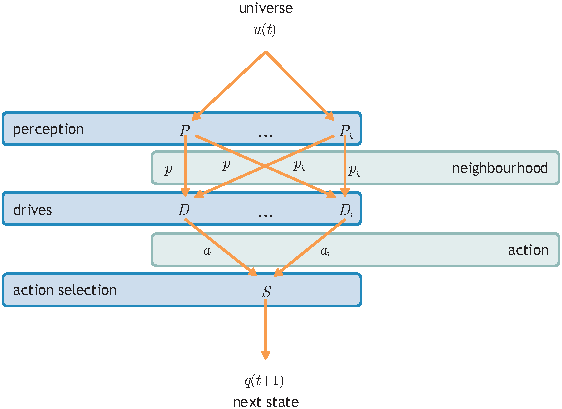
\includegraphics{fig_animat}
	\caption{The animat---the three-stage scheme of the reformulated transition function $\delta$.}
	\label{fig:animat}
\end{figure}

\begin{definition}
	\label{def:animat}
	An animat $\autom{A}=\langle\set{X},\set{Q},\set{Y},\delta,\lambda,P,D,S\rangle$ is an extended Moore automaton, where $P=\langle P_1,\ldots,P_k\rangle$, $D=\langle D_1,\ldots,D_l\rangle$, $S$ are a $k$-tuple of perception functions, an $l$-tuple of drive functions, an action selection function respectively and the transition function $\delta$ is defined as:
	\begin{eqnarray}
		& \delta(x,q) = S(\langle a_1,...,a_l\rangle,q), & \label{eq:animat:delta}\\
		& a_j = D_j(\langle p_1,...,p_k\rangle,q),\ j=1,\ldots,l, & \\
		& p_i = P_i(x,q),\ i=1,\ldots,k. & \label{eq:animat:Pi}
	\end{eqnarray}
\end{definition}

As already said, at the most basic level, the universe is a collection of inanimate and animate objects. I shall assume that it can be represented as a collection of animats (\ie\ extended Moore automata). This means that at a discrete time step $t \in \set{T}$ there are $n(t) \in \N$ animats. Nevertheless, without a loss of generality, it can be assumed that $n(t)=n,\ \forall t \in \set{T}$ and then the animats can be denoted as $\autom{A}_1,\ldots,\autom{A}_n$. 

According to the discussion at the beginning of this section, animate and inanimate objects exist in time and space. Let $\E$ be an Euclidean vector space and $\set{S}_i$ represent the set of possible internal states of animal $i$. Then, when modelling organised groups of moving animals, the state of animat $\autom{A}_i$ at a discrete time step $t \in \set{T}$ is typically represented as $q_i(t)=\langle \vect{p}_i(t), \vect{v}_i(t), s_i(t) \rangle$, where $\vect{p}_i(t) \in \E$ denotes the position in space, $\vect{v}_i(t) \in \E$ the velocity and $s_i(t) \in \set{S}_i$ the internal state of the modelled animal. 

Let $\set{Y}_i$ denote the output alphabet of animat $\autom{A}_i$ for all $i=1,\ldots,n$. It is a non-empty set representing data about animal $i$ that can be perceived by an outside observer. Therefore $\set{U}=\set{Y}_1 \times \cdots \times \set{Y}_n$ and the perceivable state of the universe at a discrete time step $t \in \set{T}$ is given by the $n$-tuple $u(t)=\langle y_1(t),\ldots,y_n(t)\rangle$, where $y_i(t)=\lambda_i(q_i(t))$ denotes the output of animat $\autom{A}_i$ at time step $t$ for all $i=1,\ldots,n$. 

At any discrete time step all animats are applied the same input; the perceivable state of the universe. In other words, at a discrete time step $t \in \set{T}$, the input that is applied to all animats is $x(t)=u(t)$. Subsequently this means that all animats use the input alphabet $\set{X}=\set{U}=\set{Y}_1 \times \cdots \times \set{Y}_n$.

If I summarize: at a discrete time step an animat is applied the current perceivable state of the universe (\ie\ the data about all of the animats that can be perceived by an outside observer). Using the transition function (\ie\ taking into consideration perception, drives and action selection), the animat computes its next discrete time step state and then emits its new output. With this the perceivable state of the universe changes. In the following sections perception, drives and action selection are going to be discussed in more detail.

%--
\subsection{Perception}
As already said, the input of an animat is the current perceivable state of the universe. Let perception be the animal's process of \emph{interpreting} the perceivable data and \emph{selecting} just the relevant information from all of the sensory signals that exist in the universe (\eg\ detect the locations of food sources in the vicinity). From the viewpoint of human perception of the universe, it could be said that there exist multiple perception types (\ie\ sight, hearing, smell, \etc), where each of them selects only the relevant information according to a specific characteristic. 

Let the current perceivable state of the universe be the $n$-tuple  $u=\langle y_1,\ldots,y_n\rangle$, where for all $i=1,\ldots,n$ $y_i \in \set{Y}_i$ is data about animat $\autom{A}_i$ that can be perceived by an outside observer. Let $q \in \set{Q}$ be the current state of the observed animat and let its input $x \in \set{X}$ be the current perceivable state of the universe, that is  $x=u=\langle y_1,\ldots,y_n \rangle$. 

Let $\N_n$ denote the set of all positive natural numbers lower or equal to $n$ and for all $i=1,\ldots,n$ let the set $\set{I}^\textnormal{c}_i$ represent information about animat $\autom{A}_i$ that can be obtained from $y_i$ with respect to a certain characteristic $\mathrm{c}$. 

Let the set $\set{N} \in \powset{\N_n}$ represent the set of indexes of members of $x$; in other words, animats that are according to characteristic $\mathrm{c}$ relevant to the observed animat. The ordered pair $p=\langle\set{N},o\rangle$, where $\set{N} \in \powset{\N_n}$ and $o \in \set{I}^\textnormal{c}_1 \times \cdots \times \set{I}^\textnormal{c}_n$ then represents the information regarding characteristic $\textnormal{c}$ that was obtained from the current perceivable state of the universe and is, with respect to this characteristic, relevant to the observed animat. For reasons of notational simplicity, let the set $\powset{\N_n} \times (\set{I}^\textnormal{c}_1 \times \cdots \times \set{I}^\textnormal{c}_n)$ be denoted simply as $\set{P}^\textnormal{c}$. 

\begin{definition}
	\label{def:animat:Pi}
	Let $x \in \set{X}$ be the current perceivable state of the universe and $p \in \set{P}^\textnormal{c}$ be the information regarding characteristic $\mathrm{c}$ that was obtained from $x$ and is, according to this characteristic and the state $q \in \set{Q}$, relevant to the animat. Then a \emph{perception function} for characteristic $\mathrm{c}$ is a mapping $P: \set{X} \times \set{Q} \mapsto \set{P}^\textnormal{c}$.
\end{definition}

For reasons of simplicity I shall address the image of a perception function with the name \emph{neighbourhood}. If I sum up, a neighbourhood obtained by means of a perception function represents only the relevant characterized sensory signals (\eg\ locations of food sources in the vicinity). This means that the perception function allows taking into account that different animals employ different strategies for sampling sensory data \cite{cliff:1993}. 

%--
\subsection{Drives}
The animal's drives are in strong correlation of its internal state and the perceived information about the state of the universe. In other words: based on the information obtained from the perceivable state of the universe (\eg\ locations of food sources in the vicinity) and its current internal state (\eg\ hunger) the animal will select actions (\eg\ feeding) that satisfy a specific \emph{drive} (\eg\ minimize hunger).

Let the observed animat have $k \in \N$ perception functions denoted as $P_1,\ldots,P_k$. This means that the set $\set{P}=\set{P}^{\mathrm{c}_1} \times \cdots \times \set{P}^{\mathrm{c}_k}$ represents information obtainable from the perceivable state of the universe. Let me for all $i=1,\ldots,k$ use $p_i \in  \set{P}^{\mathrm{c}_i}$ to denote the neighbourhood that was obtained using perception function $P_i$. Then $\langle p_1,\ldots,p_k\rangle \in \set{P}$ represents the perceived information about the current state of the universe that was, with respect to the current state of the animat, obtained from the current perceivable state of the universe. 

\begin{definition}
	\label{def:animat:Dj}
	Let $\set{A}$ denote the set of possible actions of the animat and let $a \in \set{A}$ be the action that, with respect to the perceived information about the current state of the universe $\langle p_1,\ldots,p_k\rangle \in \set{P}$ and the current state of the animat $q \in \set{Q}$, satisfies a specific drive. Then a \emph{drive function} is a mapping $D: \set{P} \times \set{Q} \mapsto \set{A}$.
\end{definition}

%--
\subsection{Action Selection}
With action selection I refer to the animal's neurological process of \emph{selecting} the \emph{sequence of muscular movements} that will accomplish the actions that result from its drives. This process must combine, prioritize, and arbitrate between potentially conflicting actions. 

Let the observed animat have $l \in \N$ drive functions denoted as $D_1,\ldots,D_l$. This means that the $l$-tuple $\langle a_1,\ldots,a_l\rangle \in \set{A}^l$ represents the animat's desired actions (\ie\ the actions that would satisfy its drives, each satisfying only one of them). 

\begin{definition}
	\label{def:animat:S}
	Let $q' \in \set{Q}$ denote the next state of the animat computed by taking into account the current state of the animat $q \in \set{Q}$ and combining, prioritizing and arbitrating between its desired actions $\langle a_1,\ldots,a_l\rangle \in \set{A}^l$. Then an \emph{action selection function} is a mapping $S: \set{A}^l \times \set{Q} \rightarrow \set{Q}$.
\end{definition}

If I sum up, at any discrete time step the animat's input is the current state of the universe. The three stage scheme of the transition function, given by equations~\eqref{eq:animat:delta}--\eqref{eq:animat:Pi}, tries to imitate the adopted theory about the behaviour of animals (\fig~\ref{fig:animat}). In the first stage the perception functions are used to retrieve, from the current perceivable state of the universe, only the information that is relevant to the observed animat. In the second stage the drive functions use the retrieved information to compute the desired actions (\ie\ those that would satisfy the observed animat's drives). Finally the action selection function combines, prioritizes and arbitrates between the potentially conflicting actions and generates the animat's next discrete time step state. 

%-----
\section{Case Study}
In the previous sections a formal definition of the animat was  presented. The animat can be used to model an inanimate or animate object. In this section I shall employ it to reproduce the computer models of bird flocking that were presented by Reynolds \cite{reynolds:1987} and Heppner and Grenander \cite{heppner:1990}. This way I will show the usability of the animat and also present the formalization of the two models. 

Reynolds based all of his processing on geometrical calculations, but even though he has published numerous works concerning his model \cite{reynolds:1987,reynolds:1993a,reynolds:1993b,reynolds:1994,reynolds:1999,reynolds:2000}, no formal definitions have ever been given. Fortunately, he has recently made available the OpenSteer library,\footnote{\href{http://opensteer.sourceforge.net}{http://opensteer.sourceforge.net}} which includes an implementation of the model. Therefore all of my studies are based on this implementation, more precisely on OpenSteer v0.8.

Heppner and Grenander, on the other hand, based their processing on stochastic differential equations. In their paper, as a contrast to Reynolds's, they give more information, but which is not sufficiently complete to allow for an immediate easy reimplementation. Furthermore, the model they used is not available on-line. Recently, however, Heppner has given me a printout of the source code of the model through personal correspondence, and thus I have based my studies on the latter. 

%--
\subsection{Formalization of Reynolds's Computer Model}
\label{subsec:animat:cwr}
Reynolds in his study \cite{reynolds:1987} modelled the universe as a collection of $n$ digital birds of the same kind and obstacles which represented inanimate objects. He states that the obstacles and the digital birds' attempts to navigate around them increase the apparent complexity of the displayed behaviour. In his paper he also suggests that the complexity of natural flocks might be due largely to the complexity of the natural environment \cite{reynolds:1987}. More recently,\footnote{\href{http://www.red3d.com/cwr/boids/applet/}{http://www.red3d.com/cwr/boids/applet/}} however, he has acknowledged that the lifelike, unpredictable behaviour of the digital birds emerges from the complex adaptive nature of the model. Furthermore, in his latest studies \cite{reynolds:1999,reynolds:2000} he states that flock-like behaviour can be achieved by using only three drives and is independent of obstacles. Thus I decided not to model the obstacles, after all, natural flocks form and exist even in open spaces, where there are no obstacles.

As already said, Reynolds's digital bird moves through the universe with a certain velocity (\ie\ flight direction and flight speed) and at every discrete time step it changes this velocity in order to approximately optimize three drives: \emph{separation}, \emph{alignment}, and \emph{cohesion} (see subsection~\ref{subsec:birdFlocks:cwr}). The decision is based purely on the digital bird's current state and the current perceivable state of the universe. More precisely, the decision is based on the perceived locations and velocities of the nearby flockmates. However, the meaning of the expression `nearby flockmates' is drive dependant. Regardless of the latter, the above led me to believe that Reynolds's digital bird could be represented as an animat \cite{lebar_bajec:2002,lebar_bajec:2003a,lebar_bajec:2003b}.

I shall assume that Reynolds's digital bird can be represented as an animat. As discussed in section~\ref{sec:animat}, the animat's internal state $q \in \set{Q}$ is defined by the triplet $\langle\vect{p},\vect{v},s\rangle$, where $\vect{p} \in \E$ is its position in space, $\vect{v} \in \E$ its velocity and $s \in \set{S}$ is the modelled animal's internal state. I shall therefore begin by defining the latter. 

\begin{definition}
	\label{def:animat:s:cwr}
	Let the triplet $r=\langle r_\textnormal{s}, r_\textnormal{a}, r_\textnormal{c}\rangle$ represent the separation, alignment and cohesion perception distances and let the triplet $\fov=\langle\fov_\textnormal{s}, \fov_\textnormal{a}, \fov_\textnormal{c}\rangle$ represent the separation, alignment and cohesion fields of view. Let $m$ represent the digital bird's mass, $v_\textnormal{M}$ its maximal achievable flight speed and $f_\textnormal{M}$ its maximal available force. Then the internal state of the animal modelled by Reynolds's digital bird is 
	\begin{equation}
	s=\langle \mathrm{r}, \fov, m, v_\textnormal{M}, f_\textnormal{M} \rangle.
	\end{equation}
\end{definition}

For reasons of simplicity it shall be assumed that only the animat's position $\vect{p}$ and velocity $\vect{v}$ change through time, while the modelled animal's internal state $s$ stays constant. This is also consistent with Reynolds's original definition \cite{reynolds:1987}. The velocity vector $\vect{v}$ gives the animat's relative position changes per coordinate axis in the Cartesian coordinate system and therefore encodes the animat's flight direction $\vect{v}^0$ and flight speed $\left\|\vect{v}\right\|$. The perception distances and fields of view define the animal's perception volume (\fig~\ref{fig:perception:cwr}). The maximal achievable speed represents a simple model of viscous speed damping (\ie\ it will be used to model the inability to exceed a certain speed even if constantly accelerating), while the maximal available force shall be used to take into account the fact that only an animal with a finite amount of energy is being modelled.

\begin{figure}
	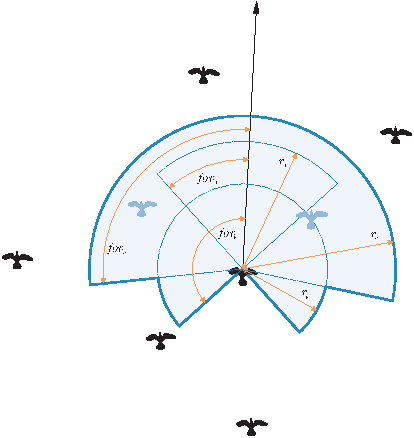
\includegraphics{fig_perception_cwr}
	\caption{The perception model that Reynolds used in the OpenSteer v0.8 implementation of his model \cite{reynolds:1999}. The black arrow represents the digital bird's flight direction. The shaded area represents the combined perception volume defined by the distinct separation ($r_\textnormal{s}$,$\fov_\textnormal{s}$), alignment ($r_\textnormal{a}$,$\fov_\textnormal{a}$) and cohesion ($r_\textnormal{c}$,$\fov_\textnormal{c}$) perception volumes. The perceived flockmates are depicted in a light blue colour.}
	\label{fig:perception:cwr}
\end{figure}

%-
\subsubsection{Modelling Perception}
As discussed before, in Reynolds's case, the universe is homogeneous (\ie\ consists of animats of the same kind). Furthermore, the number of animats is $n \in \N$ and constant through time. This means that the animat's input alphabet is $\set{X}=\set{Y}^n$. 

Let $\set{Y}=\E \times \E$ and let the animat's output function $\lambda(q)=\langle\vect{p},\vect{v}\rangle$ return the animat's current position in space and its current velocity. Then at a discrete time step $t \in \set{T}$ the perceivable state of the universe is $u(t)=\langle y_1(t),\ldots,y_n(t)\rangle$, where for all $i=1,\ldots,n$ $y_i(t)=\lambda(q_i(t))$ is the output of animat $i$ (\ie\ its position in space and its velocity) at time step $t$. 

As said, a perception function (definition~\ref{def:animat:Pi}) acts like an interpreter of the perceivable state of the universe and a selector of relevant information. Then, regarding the drives employed by Reynolds and the OpenSteer v0.8 source code, three perception functions $P_\textnormal{s}$, $P_\textnormal{a}$ and $P_\textnormal{c}$ must be defined. The separation perception function $P_\textnormal{s}$ returns the locations of the flockmates that must be avoided, the alignment perception function $P_\textnormal{a}$ returns the velocities of flockmates that should be followed and the cohesion perception function $P_\textnormal{c}$ returns the locations of flockmates that should be kept close to. 

Let $\autom{B}_i$ and $\autom{B}_j$, where $i,j \in \N_n$, be two animats from Reynolds's digital universe and let $q_j=\langle\vect{p}_j,\vect{v}_j,s_j\rangle$ be the current state of animat $\autom{B}_j$ and $y_i=\lambda(q_i)=\langle \vect{p}_i,\vect{v}_i \rangle$ be the current output of animat $\autom{B}_i$ (\ie\ the perceivable data about it). Let $\autom{B}_j$ denote the observed animat. Then the distance of animat $\autom{B}_i$ is computed as
%
\begin{equation}
	\varepsilon_i=\left\|\vect{p}_i - \vect{p}_j\right\|, \label{eq:animat:cwr:distance}
\end{equation}
%
and the direction of the offset vector between them is computed as
%
\begin{equation}
	\varphi_i=\arccos \left( \frac {\vect{v}_j \cdot (\vect{p}_i - \vect{p}_j)}{\left\| \vect{v}_j \right\| \left\| \vect{p}_i - \vect{p}_j \right\|} \right). \label{eq:animat:cwr:angularOffset}
\end{equation}

\begin{definition}
	\label{def:animat:Ps:cwr}
	Let $x=\langle y_1,\ldots,y_n\rangle$ be the current perceivable state of the universe and $j$ the index of the observed animat. Let $\set{I}^\textnormal{s}=\E$ be the set representing obtainable information about a flockmate's location. Then $\set{P}^\textnormal{s}=\powset{\N_n} \times \E^n$ and equations~\eqref{eq:animat:Ps0:cwr}--\eqref{eq:animat:Ps2:cwr} define the \emph{separation perception function} $P_\textnormal{s}: \set{X} \times \set{Q} \mapsto \set{P}^\textnormal{s}$.
	\begin{eqnarray}
		& P_\textnormal{s}(x,q)=\langle\set{N}_\textnormal{s},o_\textnormal{s}\rangle, & \label{eq:animat:Ps0:cwr} \\
		& \set{N}_\textnormal{s}=\left\{i|\ i \in \N_n,\ i \neq j,\ \varepsilon_i%(q,y_i)
		 \leq r_\textnormal{s},\ \varphi_i%(q,y_i)
		 < \fov_\textnormal{s} \right\}, & \\ 
		& o_\textnormal{s}=\langle \vect{p}_1,\ldots,\vect{p}_n\rangle. & \label{eq:animat:Ps2:cwr}
	\end{eqnarray}
\end{definition}

\begin{definition}
	\label{def:animat:Pa:cwr}
	Let $x=\langle y_1,\ldots,y_n \rangle$ be the current perceivable state of the universe and $j$ the index of the observed animat. Let $\set{I}^\textnormal{a}=\E$ be the set representing obtainable information about a flockmate's velocity. Then $\set{P}^\textnormal{a}=\powset{\N_n} \times \E^n$ and equations~\eqref{eq:animat:Pa0:cwr}--\eqref{eq:animat:Pa2:cwr} define the \emph{alignment perception function} $P_\textnormal{a}: \set{X} \times \set{Q} \mapsto \set{P}^\textnormal{a}$.
	\begin{eqnarray}
		& P_\textnormal{a}(x,q)=\langle\set{N}_\textnormal{a},o_\textnormal{a}\rangle, & \label{eq:animat:Pa0:cwr} \\
		& \set{N}_\textnormal{a}=\left\{i|\ i \in \N_n,\ i \neq j,\ \varepsilon_i%(q,y_i)
		 \leq r_\textnormal{a},\ \varphi_i%(q,y_i)
		 < \fov_\textnormal{a}\right\}, & \\ 
		& o_\textnormal{a}=\langle \vect{v}_1,\ldots,\vect{v}_n\rangle. & \label{eq:animat:Pa2:cwr}
	\end{eqnarray}
\end{definition}

\begin{definition}
	\label{def:animat:Pc:cwr}
	Let $x=\langle y_1,\ldots,y_n \rangle$ be the current perceivable state of the universe and $j$ the index of the observed animat. Let $\set{I}^\textnormal{c}=\E$ be the set representing obtainable information about a flockmate's location. Then $\set{P}^\textnormal{c}=\powset{\N_n} \times \E^n$ and equations~\eqref{eq:animat:Pc0:cwr}--\eqref{eq:animat:Pc2:cwr} define the \emph{cohesion perception function} $P_\textnormal{c}: \set{X} \times \set{Q} \mapsto \set{P}^\textnormal{c}$.
	\begin{eqnarray}
		& P_\textnormal{c}(x,q)=\langle\set{N}_\textnormal{c},o_\textnormal{c}\rangle, & \label{eq:animat:Pc0:cwr} \\
		& \set{N}_\textnormal{c}=\left\{i|\ i \in \N_n,\ i \neq j,\ \varepsilon_i%(q,y_i)
		 \leq r_\textnormal{c},\ \varphi_i%(q,y_i)
		 < \fov_\textnormal{c}\right\}, & \\
		& o_\textnormal{c}=\langle \vect{p}_1,\ldots,\vect{p}_n\rangle. & \label{eq:animat:Pc2:cwr}
	\end{eqnarray}
\end{definition}

To sum up, the three perception functions together return only those digital birds that are in the perception volume of the observed digital bird. In other words, each of the three neighbourhoods represents only the flockmates that are treated as `nearby' according to the digital bird's corresponding drive \cite{reynolds:1987} (see subsection~\ref{subsec:birdFlocks:cwr}).

%-
\subsubsection{Modelling Drives}
Recall that a drive function (definition~\ref{def:animat:Dj}), based on the current perceived information about the state of the universe and the current state of the animat, selects the action to satisfy a specific drive. Then, since Reynolds states that flock-like behaviour can be achieved if the digital bird follows three drives, three drive functions $D_\textnormal{s}$, $D_\textnormal{a}$ and $D_\textnormal{c}$ need to be defined. The separation drive function $D_\textnormal{s}$ returns the action that will keep the animat safe from colliding with the flockmates which should be avoided. The alignment drive function $D_\textnormal{a}$ returns the action that will align it with the flockmates which should be followed and the cohesion drive function $D_\textnormal{c}$ returns the action that will direct it towards the centre of the flockmates which should be kept close to. Reynolds models the drives using geometrical equations (detailed descriptions are presented in \cite{reynolds:1999}) and since he models the digital bird as a simple vehicle \cite{reynolds:1987,reynolds:1999}, he represents the desired actions as physical forces which would induce the desired flight direction and/or flight speed change.  

Let the animat's $k$-tuple of perception functions be  $P=\langle P_\textnormal{s},P_\textnormal{a},P_\textnormal{c}\rangle$. Then, according to definition~\ref{def:animat:Dj} and definitions~\ref{def:animat:Ps:cwr}--\ref{def:animat:Pc:cwr}, the set representing information obtainable from the perceivable state of the universe is $\set{P}=\set{P}^\textnormal{s} \times \set{P}^\textnormal{a} \times \set{P}^\textnormal{c}$. 

According to Reynolds \cite{reynolds:1999}, the separation drive gives the digital bird the ability to maintain a certain separation distance from nearby flockmates. In this case the nearby flockmates are the digital birds that should be avoided (\ie\ computed using the separation perception function). For each flockmate a `repulsive force' is computed by subtracting the current position of the observed animat and the current position of the flockmate. This force is then divided by the square of the flockmate's distance.\footnote{Reynolds admits \cite{reynolds:1999} that the division by the square of the flockmate's distance is just a setting that worked well and not a fundamental value.} The resulting forces are then summed together, and according to \sidenote{OpenSteer v0.8}{!animats v1.0 should first average then normalize---opensteer does so!} also normalized, to produce the desired action (\ie\ the desired change in flight direction and flight speed). 

\begin{definition}
	\label{def:animat:Ds:cwr}
	Let the current state of the animat be $q=\langle\vect{p},\vect{v},s\rangle$. Let the information that was, with respect to the current state of the animat $q$, obtained from the current perceivable state of the universe be $\langle p_\textnormal{s},p_\textnormal{a},p_\textnormal{c}\rangle \in \set{P}$ and let $p_\textnormal{s}=\langle\set{N}_\textnormal{s},o_\textnormal{s}\rangle$, where $\set{N}_\textnormal{s} \in \powset{\N_n}$ is a set representing the indexes of animats that should be avoided and $o_\textnormal{s}=\langle\vect{p}_1,\ldots,\vect{p}_n\rangle$ are their current positions in space. Let the set of available actions be $\set{A}=\E$. The \emph{separation drive function} is then the drive function $D_\textnormal{s}: \set{P} \times \set{Q} \mapsto \set{A}$ that is defined as 
	\begin{equation}
		D_\textnormal{s}(\langle p_\textnormal{s},p_\textnormal{a},p_\textnormal{c}\rangle, q) = \left[ \sum_{i \in \set{N}_\textnormal{s}} \frac{\vect{p}-\vect{p}_i}{{\left\|\vect{p}_i-\vect{p}\right\|}^2} \right]^0. \label{eq:animat:Ds:cwr}
	\end{equation}
\end{definition}

The alignment drive, on the other hand, gives the digital bird the ability to align itself with (\ie\ fly in the same flight direction and/or with the same speed as) the nearby flockmates. The nearby flockmates in this case are the digital birds that should be followed. The average of the velocities of these flockmates is computed and represents the desired new velocity of the observed digital bird. The velocity difference is computed by subtracting the observed digital bird's velocity from the desired new velocity. Finally the force representing the desired action is then, according to OpenSteer v0.8, computed by normalizing the velocity difference.

\begin{definition}
	\label{def:animat:Da:cwr}
	Let the current state of the animat be $q=\langle\vect{p},\vect{v},s\rangle$. Let the information that was, with respect to the current state of the animat $q$, obtained from the current perceivable state of the universe be $\langle p_\textnormal{s},p_\textnormal{a},p_\textnormal{c}\rangle \in \set{P}$ and let $p_\textnormal{a}=\langle\set{N}_\textnormal{a},o_\textnormal{a}\rangle$, where $\set{N}_\textnormal{a} \in \powset{\N_n}$ is a set representing the indexes of animats that should be followed and $o_\textnormal{a}=\langle\vect{v}_1,\ldots,\vect{v}_n\rangle$ are their current velocities. Let the set of available actions be $\set{A}=\E$. The \emph{alignment drive function} is then the drive function $D_\textnormal{a}: \set{P} \times \set{Q} \mapsto \set{A}$ that is defined as 
	\begin{equation}
		D_\textnormal{a}(\langle p_\textnormal{s},p_\textnormal{a},p_\textnormal{c}\rangle, q) = \left[ \Biggl( \frac{1}{\left|\set{N}_\textnormal{a}\right|} \sum_{i \in \set{N}_\textnormal{a}} \vect{v}_i \Biggr) - \vect{v} \right]^0. \label{eq:animat:Da:cwr}
	\end{equation}
\end{definition}

Finally, the cohesion drive gives the digital bird the ability to cohere with (\ie\ approach and form a group with) the nearby flockmates. Here the nearby flockmates are the digital birds that should be kept close to. The centre (\ie\ the \emph{centre of mass} or \emph{average position}) of these flockmates is computed and represents the desired position of the observed digital bird. The `attraction force' is computed by subtracting the observed digital bird's position from the desired position. At last the force representing the desired action is, according to OpenSteer v0.8, computed by normalizing the attraction force.

\begin{definition}
	\label{def:animat:Dc:cwr}
	Let the current state of the animat be $q=\langle\vect{p},\vect{v},s\rangle$. Let the information that was, with respect to the current state of the animat $q$, obtained from the current perceivable state of the universe be $\langle p_\textnormal{s},p_\textnormal{a},p_\textnormal{c}\rangle \in \set{P}$ and let $p_\textnormal{c}=\langle\set{N}_\textnormal{c},o_\textnormal{c}\rangle$, where $\set{N}_\textnormal{c} \in \powset{\N_n}$ is a set representing the indexes of animats that should be kept close to and $o_\textnormal{c}=\langle\vect{p}_1,\ldots,\vect{p}_n\rangle$ are their current positions in space. Let the set of available actions be $\set{A}=\E$. The \emph{cohesion drive function} is then the drive function $D_\textnormal{c}: \set{P} \times \set{Q} \mapsto \set{A}$ that is defined as 
	\begin{equation}
		D_\textnormal{c}(\langle p_\textnormal{s},p_\textnormal{a},p_\textnormal{c}\rangle, q) = \left[ \left( \frac{1}{\left|\set{N}_\textnormal{c}\right|} \sum_{i \in \set{N}_\textnormal{c}} \vect{p}_i \right) - \vect{p} \right]^0. \label{eq:animat:Dc:cwr}
	\end{equation}
\end{definition}

%-
\subsubsection{Modelling Action Selection}
Each of the three drive functions returns a physical force that would satisfy the specific drive. Recall that the action selection function (definition~\ref{def:animat:S}), combines, prioritizes and arbitrates between potentially conflicting actions to select the sequence of muscular movements that will eventually accomplish all of the animal's drives. In his original study Reynolds \cite{reynolds:1987} proposes that the physical forces should be combined using a special algorithm named \emph{prioritized acceleration allocation}. But in one of his later studies \cite{reynolds:1999} he also admits that in the course of several reimplementations of the model over the years, a simpler linear combination has proved sufficient. Moreover, in his latest implementation in OpenSteer v0.8 he uses a weighted sum combination. 

This means that Reynolds models action selection as a weighted sum of the desired actions (\ie\ weighted sum of the respective physical forces). The resulting force is used to compute the digital bird's new position in space and velocity. This computation is subjected to a set of constraints modelling conservation of momentum, viscous damping and the animal's finite amount of energy. He names the approach \emph{geometrical flight} \cite{reynolds:1987}.

\sidenote{Reynolds does not model the musculoskeletal structure of a bird}{v1.1.20050210 [FHH]: this may be a very unrealistic assumption---birds, like air planes, have stability-producing features that make them tend to go in a straight line unless positively directed otherwise.\\v1.3.20050402 [ILB]: This is taken care of by geometrical flight.}, but models it as a point mass vehicle \cite{reynolds:1987,reynolds:1999}. This means that the animat's physics is based on forward Euler integration. In other words, the combined forces (limited by the animat's maximal available force) are applied to the animat's point mass. This produces an acceleration equal to the combined force divided by the animat's mass. The acceleration is then added to the animat's current velocity and truncated by the maximum achievable speed. Finally the animat's new position in space is computed by adding the new velocity to the animat's current position in space.

Let $\vect{a} \in \E$ be a vector and let $a \in \R^+$ represent the maximal size of $\vect{a}$. Then the truncation of vector $\vect{a}$ to its maximal size $a$ is calculated as
%
\begin{equation}
	\lfloor\vect{a}\rceil^{a} = \min(\left\|\vect{a}\right\|, a) \vect{a}^0. \label{eq:truncation}
\end{equation}

\begin{definition}
	\label{def:animat:Sws:cwr}
	Let the current state of the animat be $q=\langle\vect{p},\vect{v},s\rangle$, where the modelled animal's internal state $s$ is defined by definition~\ref{def:animat:s:cwr}. Let the $l$-tuple of drive functions be $D=\langle D_\textnormal{s}, D_\textnormal{a}, D_\textnormal{c}\rangle$ and let the computed desired actions be $\langle a_\textnormal{s},a_\textnormal{a},a_\textnormal{c}\rangle$. Let $w_\textnormal{s}$, $w_\textnormal{a}$ and $w_\textnormal{c}$ represent the weights of the separation, alignment and cohesion drive respectively and let $dt$ represent the simulation step. Then the \emph{weighted sum action selection function} is the action selection function $S_\textnormal{ws}: \set{A} \times \set{Q} \mapsto \set{Q}$ that is defined as
	\begin{equation}
		S_\textnormal{ws}(\langle a_\textnormal{s},a_\textnormal{a},a_\textnormal{c}\rangle, q) = \langle\vect{p}', \vect{v}', s\rangle, \label{eq:animat:Sws0:cwr}
	\end{equation}
	\vspace{-3mm}
	\begin{equation}
		\vect{v}' = \left\lfloor {\vect{v} + \frac{\left\lfloor w_\textnormal{s}a_\textnormal{s} + w_\textnormal{a}a_\textnormal{a} + w_\textnormal{c}a_\textnormal{c} \right\rceil^{f_\textnormal{M}}}{m}}dt \right\rceil^{v_\textnormal{M}},
	\end{equation}
	\vspace{-3mm}
	\begin{equation}
		\vect{p}' = \vect{p} + \vect{v}'dt. \label{eq:animat:Sws2:cwr}
	\end{equation}
\end{definition}

Therefore Reynolds's digital bird can be defined as a special animat. 

\begin{definition}
	\label{def:animat:cwr}
	Reynolds's digital bird is the animat $\autom{B}=\langle\set{X},\set{Q},\set{Y},\delta,\lambda,P,D,S\rangle$. The set representing internal states is $\set{Q}=\E \times \E \times \set{S}$, where $\set{S}$ is defined by definition~\ref{def:animat:s:cwr}. The output alphabet is $\set{Y}=\E \times \E$ and the input alphabet is $\set{X}=\set{Y}^n$. The animat's current internal state $q=\langle\vect{p},\vect{v},s\rangle$ represents the modelled animal's current position in space $\vect{p} \in \E$, velocity $\vect{v} \in \E$ and internal state $s \in \set{S}$. The output function $\lambda: \set{Q} \mapsto \set{Y}$ is $\lambda(q)=\langle\vect{p},\vect{v}\rangle$. The $k$-tuple of perception functions is $P=\langle P_\textnormal{s},P_\textnormal{a},P_\textnormal{c}\rangle$, where $P_\textnormal{s}$, $P_\textnormal{a}$ and $P_\textnormal{c}$ are the separation, alignment and cohesion perception function respectively (definitions~\ref{def:animat:Ps:cwr}--\ref{def:animat:Pa:cwr}). The $l$-tuple of drive functions is $D=\langle D_\textnormal{s},D_\textnormal{a},D_\textnormal{c}\rangle$, where $D_\textnormal{s}$, $D_\textnormal{a}$ and $D_\textnormal{c}$ are the separation, alignment and cohesion drive function respectively (definitions~\ref{def:animat:Ds:cwr}--\ref{def:animat:Dc:cwr}). Finally, the action selection function is the weighted sum action selection function $S=S_\textnormal{ws}$ (definition~\ref{def:animat:Sws:cwr}).
\end{definition}

%--
\subsection{Formalization of Heppner and Grenander's Computer Model}
\label{subsec:animat:fhh}
Heppner and Grenander in their study \cite{heppner:1990} modelled the universe as a collection of $n$ digital birds of the same kind. As a contrast to Reynolds they did not model any obstacles, but added a special influence modelling random distractions. Furthermore, they admit that without this influence they were not able to achieve flock-like behaviour.

Nevertheless, all things considered, they had a similar approach as Reynolds. Their digital bird moves through the universe with a certain velocity and at every discrete time step it changes this velocity in order to satisfy three drives: \emph{homing}, \emph{velocity regulation}, and \emph{interaction} (see subsection~\ref{subsec:birdFlocks:fhh}). The decision is again based purely on the digital bird's current state and the current perceivable state of the universe. More precisely the decision is based on the digital bird's position, velocity and the perceived locations of the nearby flockmates. 

Let me define the animat that models Heppner and Grenander's digital bird. As discussed in section~\ref{sec:animat}, the animat's internal state $q \in \set{Q}$ is defined by the triplet $\langle \vect{p}, \vect{v}, s \rangle$, where $\vect{p} \in \E$ is its position in space, $\vect{v} \in \E$ its velocity and $s \in \set{S}$ is the modelled animal's internal state. Let me again first define the latter. 

\begin{definition}
	\label{def:animat:s:fhh}
	Let $\vect{r} \in \E$ be the position of the centre of the roosting area of the the modelled bird, $r_\textnormal{o}$ its perception range, $v_\textnormal{p}$ its preferred flight speed and $d_\textnormal{p}$ its preferred distance from flockmates. Then the internal state of the animal modelled by Heppner and Grenander's digital bird is
	\begin{equation}
		s=\langle \vect{r}, r_\textnormal{o}, v_\textnormal{p}, d_\textnormal{p} \rangle.
	\end{equation}
\end{definition}

As in Reynold's case (subsection~\ref{subsec:animat:cwr}) I shall assume that only the animat's position $\vect{p}$ and $\vect{v}$ can change through time, while the 	modelled animal's internal state $s$ stays constant. This is again consistent with Heppner and Grenander's original definition \cite{heppner:1990}. The velocity vector $\vect{v}$ is thus again used to encode the flight direction $\vect{v}^0$ and flight speed $\left\|\vect{v}\right\|$. The perception range defines an omnidirectional perception volume (\fig~\ref{fig:perception:fhh}).

\begin{figure}
	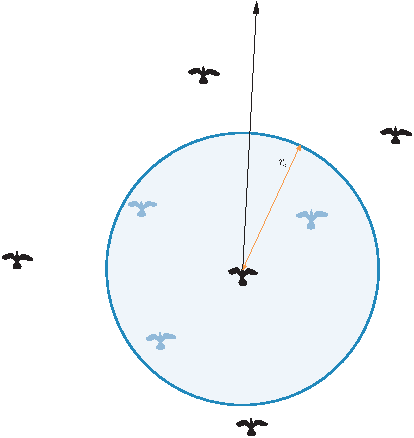
\includegraphics{fig_perception_fhh}
	\caption{The perception model used by Heppner and Grenander \cite{heppner:1990}. The black arrow represents the digital bird's flight direction. The shaded area represents the omnidirectional perception volume defined by the perception range. The perceived flockmates are depicted in a light blue colour.}
	\label{fig:perception:fhh}
\end{figure}

The preferred flight speed is the flight speed to which the bird wishes to return if perturbed and the preferred distance defines the optimal distance from a flockmate (\ie\ the distance at which the bird is neither attracted to nor repulsed from the flockmate).

%-
\subsubsection{Modelling Perception}
As discussed before, in Heppner and Grenander's case the universe again consists of animats of the same kind. Similarly, their number $n \in \N$ is constant through time, which means that the animat's input alphabet is yet again $\set{X}=\set{Y}^n$.

For reasons of consistency let the output alphabet again be $\set{Y}=\E \times \E$ and let the animat's output function $\lambda(q)=\langle\vect{p},\vect{v}\rangle$ return the animat's current position in space and velocity. Even in Heppner and Grenander's case the perceivable state of the universe at a discrete time step $t \in \set{T}$ is $u(t)=\langle y_1(t),\ldots,y_n(t)\rangle$, where for all $i=1,\ldots,n$ $y_i(t)=\lambda(q_i(t))$ is the output of animat $i$ (\ie\ its position in space and its velocity) at time step $t$. 

Recall from subsection~\ref{subsec:birdFlocks:fhh} that Heppner and Grenander gave their digital bird full and precise knowledge about the locations of all surrounding digital birds that are closer than a predefined distance. Let $\autom{B}_i$ and $\autom{B}_j$, where $i, j \in \N_n$, be two animats from Heppner and Grenander's digital universe and let the current state of animat $\autom{B}_j$ be $q_j=\langle \vect{p}_j,\vect{v}_j,s_j \rangle$ and the current perceivable data about animat $\autom{B}_i$ be $y_i=\langle \vect{p}_i, \vect{v}_i \rangle$. Let $\autom{B}_j$ denote the observed animat. Then recall from equation~\eqref{eq:animat:cwr:distance} that the distance of animat $\autom{B}_i$ from the observed animat $\autom{B}_j$ is computed as
%
\begin{equation}
	\varepsilon_i=\left\|\vect{p}_i - \vect{p}_j\right\|. \nonumber
\end{equation}

\begin{definition}
	\label{def:animat:Po:fhh}
	Let $x=\langle y_1,\ldots,y_n\rangle$ be the current perceivable state of the universe and $j$ the index of the observed animat. Let $\set{I}^\textnormal{o}=\E$ be the set representing obtainable information about a flockmate's location. Then $\set{P}^\textnormal{o}=\powset{\N_n} \times \E^n$ and equations~\eqref{eq:animat:Po0:fhh}--\eqref{eq:animat:Po2:fhh} define the \emph{omnidirectional perception function} $P_\textnormal{o}: \set{X} \times \set{Q} \mapsto \set{P}^\textnormal{o}$.
	\begin{eqnarray}
		& P_\textnormal{o}(x,q)=\langle\set{N}_\textnormal{o},o_\textnormal{o}\rangle, & \label{eq:animat:Po0:fhh} \\
		& \set{N}_\textnormal{o}=\left\{i|\ i \in \N_n,\ i \neq j,\ \varepsilon_i \leq r_\textnormal{o} \right\}, & \\ 
		& o_\textnormal{o}=\langle \vect{p}_1,\ldots,\vect{p}_n\rangle. & \label{eq:animat:Po2:fhh}
	\end{eqnarray}
\end{definition}

%-
\subsubsection{Modelling Drives}
Recall from subsection~\ref{subsec:birdFlocks:fhh} that homing expresses the bird's tendency to stay in a roosting area and depends only on the digital bird's current position. Velocity regulation expresses its tendency to fly with a certain flight speed and depends only on the digital bird's current flight speed. Finally interaction expresses the bird's attraction to or repulsion from flockmates and depends only on the perceived locations of the nearby flockmates. 

Let the animat employ only the omnidirectional perception function. Then $P=\langle P_\textnormal{o} \rangle$ and, according to definitions~\ref{def:animat:Dj} and \ref{def:animat:Po:fhh}, the set representing information obtainable from the perceivable state of the universe is $\set{P}=\set{P}^\textnormal{o}$.

\begin{definition}
	\label{def:animat:Dh:fhh}
	Let the current state of the animat be $q=\langle\vect{p},\vect{v},s\rangle$, where the modelled animal's internal state is $s=\langle\mathrm{r},r_\textnormal{o},v_\textnormal{p},d_\textnormal{p}\rangle$ as defined by definition~\ref{def:animat:s:fhh}. Let $p_\textnormal{o}$ denote the neighbourhood obtained by using the omnidirectional perception function. Let the set of available actions be $\set{A}=\E$. Let $h_\textnormal{m}$ be the minimum distance for roost attraction and $h_\textnormal{M}$ the distance of maximum roost attraction. The \emph{homing drive function} is then the drive function $D_\textnormal{h}: \set{P} \times \set{Q} \mapsto \set{A}$ that is defined as 
	\begin{equation}
		D_\textnormal{h}(p_\textnormal{o}, q) = \left\{
		\begin{array}{ll}
		\vect{0} & \mathrm{iff}\ \left\|\vect{r}-\vect{p}\right\| < h_\textnormal{m} \\
		\frac{c^a \mathrm{e}^{-bc}}{\left(a/b\right)^a \mathrm{e}^{-a}} \left(\vect{r}-\vect{p}\right)^0  & \mathrm{iff}\ \left\|\vect{r}-\vect{p}\right\| \geq h_\textnormal{m}
		\end{array}
		\right., \label{eq:animat:Dr:fhh}
	\end{equation}
	where $a$ and $b$ are parameters for controlling the shape of the attraction function and 
	\begin{equation}
		c=\frac{a}{b}\left(\frac{\left\|\vect{r}-\vect{p}\right\|-h_\textnormal{m}}{h_\textnormal{M}}\right).
	\end{equation}
\end{definition}

\begin{definition}
	\label{def:animat:Dv:cwr}
	Let the current state of the animat be $q=\langle\vect{p},\vect{v},s\rangle$, where the modelled animal's internal state is $s=\langle\mathrm{r},r_\textnormal{o},v_\textnormal{p},d_\textnormal{p}\rangle$ as defined by definition~\ref{def:animat:s:fhh}. Let $p_\textnormal{o}$ denote the neighbourhood obtained by using the omnidirectional perception function and let the set of available actions be $\set{A}=\E$. The \emph{velocity regulation drive function} is then the drive function $D_\textnormal{v}: \set{P} \times \set{Q} \mapsto \set{A}$ that is defined as 
	\begin{equation}
		D_\textnormal{v}(p_\textnormal{o}, q) = \left(v_\textnormal{p}-\left\|\vect{v}\right\|\right)\vect{v}^0. \label{eq:animat:Dv:fhh}
	\end{equation}
\end{definition}

\begin{definition}
	\label{def:animat:Di:fhh}
	Let the current state of the animat be $q=\langle\vect{p},\vect{v},s\rangle$, where the modelled animal's internal state is $s=\langle\mathrm{r},r_\textnormal{o},v_\textnormal{p},d_\textnormal{p}\rangle$ as defined by definition~\ref{def:animat:s:fhh}. Let the neighbourhood obtained by using the omnidirectional perception function be $p_\textnormal{o}=\langle\set{N}_\textnormal{o},o_\textnormal{o}\rangle$, where $\set{N}_\textnormal{o} \in \powset{\N_n}$ is the set of indexes of relevant animats and $o_\textnormal{o}=\langle\vect{p}_1,\ldots,\vect{p}_n\rangle$ are their locations. Let the set of available actions be $\set{A}=\E$ and let $f_\textnormal{M}$ denote the maximal repulsion force. The \emph{interaction drive function} is then the drive function $D_\textnormal{i}: \set{P} \times \set{Q} \mapsto \set{A}$ that is defined as 
	\begin{equation}
		D_\textnormal{i}(p_\textnormal{o}, q) = \sum_{i \in \set{N}_\textnormal{o}} \left[1-\frac{(\left\|\vect{p}_i-\vect{p}\right\|-a)^2}{b}\right] c \left(\vect{p}_i-\vect{p}\right)^0, \label{eq:animat:Di:fhh}
	\end{equation}
	where $a=\frac{d_\textnormal{p}+r_\textnormal{o}}{2}$, $b=\left(\frac{d_\textnormal{p}-r_\textnormal{o}}{2}\right)^2$ and 
	\begin{equation}
		c = \left\{
		\begin{array}{ll}
			1 & \mathrm{iff}\ \left\|\vect{p}_i-\vect{p}\right\| \geq d_\textnormal{p} \\
			\left\|\vect{p}_i-\vect{p}\right\|\frac{(b-a^2)-f_\textnormal{M}}{d_\textnormal{p}(b-a^2)}+\frac{f_\textnormal{M}b}{b-a^2} & \mathrm{iff}\ \left\|\vect{p}_i-\vect{p}\right\| < d_\textnormal{p}
		\end{array}
		\right..
	\end{equation}
\end{definition}

%-
\subsubsection{Modelling Action Selection}
Each of the three drive functions returns a vector which may be interpreted as an unconventional (non-Newtonian) \cite{heppner:1990} force that would satisfy the specific drive. Recall that the action selection function (definintion~\ref{def:animat:S}) combines, prioritizes and arbitrates between these potentially conflicting forces. Heppner and Grenander again took a similar approach as Reynolds and modelled action selection as a simple weighted sum. However, apart from the Poisson stochastic process modelling the effects of wind gusts and random local disturbances they did not apply any additional constraints.

\begin{definition*}
	\label{def:animat:Ss:fhh}
	Let the current state of the animat be $q=\langle\vect{p},\vect{v},s\rangle$. Let the $l$-tuple of drive functions be $D=\langle D_\textnormal{h}, D_\textnormal{v}, D_\textnormal{i}\rangle$ (definitions~\ref{def:animat:Dh:fhh}--\ref{def:animat:Di:fhh}) and let the computed desired actions be $\langle a_\textnormal{h},a_\textnormal{v},a_\textnormal{i}\rangle$. Let $w_\textnormal{h}$, $w_\textnormal{v}$ and $w_\textnormal{i}$ represent the weights of the homing, velocity regulation and interaction drive respectively and let $dt$ represent the simulation step. Then the \emph{simple weighted sum action selection function} is the action selection function $S_\textnormal{s}: \set{A} \times \set{Q} \mapsto \set{Q}$ that is defined as
	\begin{eqnarray}
		& S_\textnormal{s}(\langle a_\textnormal{h},a_\textnormal{v},a_\textnormal{i}\rangle, q) = \langle\vect{p}', \vect{v}', s\rangle, & \label{eq:animat:Ss0:fhh} \\
		& \vect{p}' = \vect{p} + \vect{v}dt, & \\
		& \vect{v}' = \vect{v} + \left(w_\textnormal{h}a_\textnormal{h} + w_\textnormal{v}a_\textnormal{v} + w_\textnormal{i}a_\textnormal{i}\right)dt + \vect{d}dt, & \label{eq:animat:Ss2:fhh} 
	\end{eqnarray}
	where $\vect{d} \in \E$ is a Poisson controlled vector modelling random distractions.
\end{definition*}

Heppner and Grenander's digital bird \cite{heppner:1990} is therefore a special animat.

\begin{definition}
	\label{def:animat:fhh}
	The animat modelling Heppner and Grenander's digital bird is the animat $\autom{B}=\langle\set{X},\set{Q},\set{Y},\delta,\lambda,P,D,S\rangle$. The set representing internal states is $\set{Q}=\E \times \E \times \set{S}$, where $\set{S}$ is defined by definition~\ref{def:animat:s:fhh}. The output alphabet is $\set{Y}=\E \times \E$ and the input alphabet is $\set{X}=\set{Y}^n$. The animat's current internal state $q=\langle\vect{p},\vect{v},s\rangle$ represents the modelled animal's current position in space $\vect{p} \in \E$, velocity $\vect{v} \in \E$ and internal state $s \in \set{S}$. The output function $\lambda: \set{Q} \mapsto \set{Y}$ is $\lambda(q)=\langle\vect{p},\vect{v}\rangle$. The $k$-tuple of perception functions is $P=\langle P_\textnormal{o}\rangle$, where $P_\textnormal{o}$ is the omnidirectional perception function (definition~\ref{def:animat:Po:fhh}). The $l$-tuple of drive functions is $D=\langle D_\textnormal{h},D_\textnormal{v},D_\textnormal{i}\rangle$, where $D_\textnormal{h}$, $D_\textnormal{v}$ and $D_\textnormal{i}$ are the homing, velocity regulation and interaction drive function respectively (definitions~\ref{def:animat:Dh:fhh}--\ref{def:animat:Di:fhh}). The action selection function is the simple weighted sum action selection function $S=S_\textnormal{s}$ (definition~\ref{def:animat:Ss:fhh}).
\end{definition}
